
\documentclass[12pt]{article}
\thispagestyle{empty}
\usepackage{amsmath}
\usepackage[margin=1in]{geometry}
\usepackage{amsfonts}
\usepackage{hyperref}
\usepackage{graphicx}
\usepackage{siunitx}
\usepackage{cancel}
\usepackage{xfrac}
\usepackage{listings}

\begin{document}
\begin{center}
	\par\noindent \large Logical Bit Shifts  [ Andy Chong Sam ]
\end{center}
\section{Logical Left Shift}
	\begin{minipage}[t]{.5\linewidth}		
\textbf{(I)} Consider the following  line of Java code: 
\begin{flalign*}
	\text{int }i = 20 << 1;
\end{flalign*}
\par\noindent The value of \(i\) is 40. A logical left shift by one doubles a number.
\newline
\newline
\textbf{(II)} In binary, 20 is represented as \textbf{10100}. The image below shows this representation along with the place numbers at the bottom:
\begin{center}
	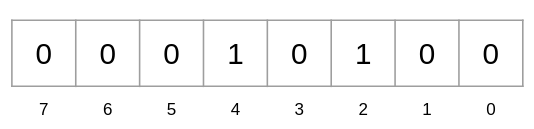
\includegraphics[width=6.5cm]{20bin.png}
\end{center}
\par\noindent We can confirm that this is correct since:
\begin{flalign*}
	1(2)^4 + 1(2)^2 = 20 
\end{flalign*}

\par\noindent \textbf{(III)} If we do a left shift, the most significant bit is discarded and a 0 is placed in position zero:
\begin{center}
	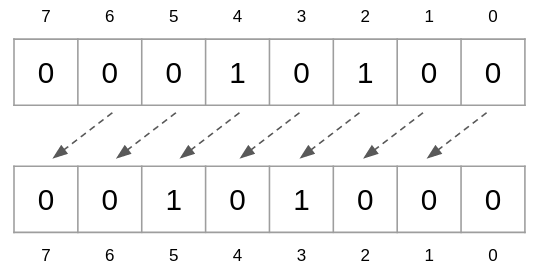
\includegraphics[width=6.5cm]{20bin-left.png}
\end{center}
\par\noindent The decimal value is now:
\begin{flalign*}
	1(2)^5 + 1(2)^3 = 40
\end{flalign*}
\par\noindent Let's see why this works.


	
\end{minipage}
\hspace{0.35cm}
\begin{minipage}[t]{.5\linewidth} 
\par\noindent \textbf{(IV)} Suppose that a decimal number is calculated from three binary digits. Let d be the binary digit. Let \(a\), \(b\), and \(c\) represent arbitrary bit positions. If \(x\) is the decimal representation of the number then:
\begin{flalign*}
x = d_a\;(2)^a + d_b\;(2)^b + d_c\;(2)^c
\end{flalign*}
\newline
\par\noindent A left shift shifts the position of \(a\), \(b\), and \(c\) by one, so the new decimal \(y\) would be:
\begin{flalign*}
	y = d_{a}\;(2)^{a+1} + d_{b}\;(2)^{b+1} + d_{c}\;(2)^{c+1}
\end{flalign*}
\newline
\par\noindent By the power rule for products we can rewrite this as:
\begin{flalign*}
	y = d_{a}\;(2^a)\;(2) + d_{b}\;(2^b)\;(2) + d_{c}\;(2^c)\;(2) \\\text{If we factor out the 2:} \\
	y = 2(\;d_{a}\;(2)^a + d_{b}\;(2)^b + d_{c}\;(2)^c\;)
\end{flalign*}
\newline
\par\noindent We can see that \(y=2x\), so a left shift by one position has the effect of doubling a decimal number.
\newline
\par\noindent \textbf{(V)} Let's see what happens when we generalize this shift to \(n\) positions to the left:
\begin{flalign*}
	y = d_{a}\;(2)^{a+n} + d_{b}\;(2)^{b+n} + d_{c}\;(2)^{c+n} \\
	y = d_{a}\;(2^a)\;(2^n) + d_{b}\;(2^b)\;(2^n) + d_{c}\;(2^c)\;(2^n) \\
	2^n(\;d_{a}\;(2)^a + d_{b}\;(2)^b + d_{c}\;(2)^c\;)
\end{flalign*}
\newline
\par\noindent So a shift of \(n\) positions to the left is equivalent to multiplying the original number by \(2^n\).
\end{minipage}
\newpage
\thispagestyle{empty}
\section{Logical Right Shift}
	\begin{minipage}[t]{.5\linewidth}		
\par\noindent\textbf{(I)} Now consider the following: 
\begin{flalign*}
	\text{int } j = 20 >>> 1;
\end{flalign*}
\par\noindent The value of \(j\) is 10.  A logical right shift by one halves a number.
\newline
\par\noindent In a right shift the least significant bit is discarded, and a zero is placed in the most significant bit.
\newline
\begin{center}
	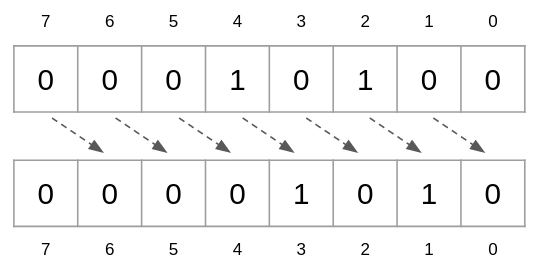
\includegraphics[width=6.5cm]{20bin-right.png}
\end{center}		
	
	\par \noindent We can see that the new value is 10:
	\begin{flalign*}
		1(2)^3 + 1(2)^1 = 10
	\end{flalign*}
		\par\noindent Just like with the left shift, we can show how shifting right works mathematically. We'll use the same generic decimal number from the previous section:
		\begin{flalign*}
			x = d_a\;(2)^a + d_b\;(2)^b + d_c\;(2)^c
		\end{flalign*}
		
\end{minipage}
	\hspace{0.35cm}
	\begin{minipage}[t]{.5\linewidth}		
\par\noindent \textbf{(II)}  A shift to the right would decrease the value of the exponents by one.
\begin{flalign*}
	y = d_{a}\;(2)^{a-1} + d_{b}\;(2)^{b-1} + d_{c}\;(2)^{c-1}
\end{flalign*}
\par\noindent Using the quotient rule:
\begin{flalign*}
	y = d_{a}\;(2)^{a-1} + d_{b}\;(2)^{b-1} + d_{c}\;(2)^{c-1} \\
	y = d_{a}\;\frac{2^a}{2} + d_{b}\;\frac{2^b}{2} + d_{c}\frac{2^c}{2} \\
	\text{If we factor out the \(\frac{1}{2}\)}: \\
	y=\frac{\;d_{a}\;(2)^a + d_{b}\;(2)^b + d_{c}\;(2)^c\;}{2}
\end{flalign*}
\newline
\par\noindent Since \(y=\frac{x}{2}\), a right shift by one position has the effect of halving a decimal number.
\newline
\par\noindent \textbf{(III)} Finally, let's generalize for \(n\) shifts to the right:
\begin{flalign*}
	y = d_{a}\;(2)^{a-n} + d_{b}\;(2)^{b-n} + d_{c}\;(2)^{c-n} \\
		y = d_{a}\;\frac{2^a}{2^n} + d_{b}\;\frac{2^b}{2^n} + d_{c}\frac{2^c}{2^n} \\
		y = \frac{\;d_{a}\;(2)^a + d_{b}\;(2)^b + d_{c}\;(2)^c\;}{2^n}
\end{flalign*}
\newline
\par\noindent So a shift of \(n\) to the right is equivalent to dividing the original number by \(2^n\).

\end{minipage}



\end{document}